The work within \textsc{Realdark} proposal builds novel data acquisition and selection tools and techniques in WP1 and applies them to obtain the physics results in WP2-4. This modus operandi follows my proven track record of bringing challenging improvements to the data taking system and to the combined performance of the entire experiment, and successfully exploiting them for world-best physics measurements and searches. 

Sec.~\ref{sub:CommonMethodsTechnicalTools} and Sec.~\ref{sub:CommonMethodsAnalysisTools} describe the common methodologies required for reaching the objectives of the WPs described in Sec.~\ref{sub:objectives}. 
Their description follows logically the procedures designed to record, treat and analyze large amounts of raw data towards the dissemination of results that can shed light on the particle nature of DM. Specific methodologies are described in Sec.~\ref{sub:SpecificMethodsCompression}. 

How all these methods fit together in the project planning is described in Sec.~\ref{sub:ProjectPlanning}.  

\subsection{Methodologies: technical tools}
\label{sub:CommonMethodsTechnicalTools}

\subsubsection{Common methodologies: From LHC collisions to physics objects for analysis}
\label{subsub:TriggerRecoSoftware}

%Should I have "my expertise" here or in project planning? For now, here. 
In this section outlines the methods used to record data with the techniques proposed, 
and transform these data into physics quantities to be used for the searches in WP2-4. 

\textbf{From LHC collisions to storage} The ATLAS core software infrastructure receives raw trigger and detector information from collisions and assembles it into different data streams. 
Full events that passed the selections determined by the ATLAS trigger menu are placed in the \texttt{physics\_Main} stream for subsequent reconstruction, while partially-built detector data (including TLA and TLA+PEB objects) need to be selected by dedicated software algorithms and placed in specific data streams. 
In WP1, I will rely on my expertise as one of the main authors of the TLA framework in Run-2, and deploy new multithreaded software algorithms that can write out jets, photons, muons and electrons, as well as user-defined partial detector information. 
These algorithms are executed if an event is selected by a given L1+HLT trigger "\textit{seed}" chain, in order to reduce the storage and CPU cost of downstream HLT algorithms. 
Given that a large part of the searches in this proposal occurs at the HLT, a resource constrained environment, an important part of the planning prior to data taking is to optimize the CPU and storage resources needed for each of the planned data streams, based on the sensitivity of the searches in WP2-4. 
We will compare storage and CPU costs~\cite{ToBeCited} % CostMonitoring talk by Tim 
of different seed chain options, to make an informed decision for the TLA and TLA+PEB streams. 

\textbf{Reconstruction} Full events are passed through the ATLAS reconstruction software, so that raw detector data can be reconstructed into final physics objects (muons, electrons, jets...). 
While TLA events are already reconstructed within the HLT software using inputs and algorithms that are as close as possible to offline, 
TLA+PEB events require the offline software reconstruction algorithms to be adapted, to cope with receiving partial detector data as input. 
We can take advantage of trigger-level reconstruction algorithms, where regional reconstruction has already been used to optimize HLT resources~\cite{ToBeCited}, %Partial event building
and extend existing reconstruction and identification techniques to non-isolated muons and electrons in hadronic environments~\cite{ToBeCited}. %Muons in b-jets, heavy neutrinos, and Tuhin Roy's paper

\textbf{Object identification and calibration} Correct object identification and calibration is a crucial point to be able to use HLT and custom objects for physics analysis.
I am an expert of jet calibration 
In the case of TLA, these can be improved at a later date using dedicated algorithms and more refined corrections that are not applied at the HLT. 
Relying on the success of HLT jet calibration in my StG, we will keep the procedures to identify and calibrate HLT objects in this proposal as close as possible to those of offline objects, with additional data-derived corrections and scale-factors applied to HLT objects covering the remaining differences. 
%Tracking: where do we need it? Jets, mostly.
A major improvement in the Run-3 calibration procedures is the addition of tracking information computed by the HLT software, as described in Sec.~\ref{sub:stateOfTheArtExperiment}. 
This allows for improvements in both jet reconstruction and calibration, as \textit{particle flow}~\cite{ToBeCited} %cite: PFlow
jets combining calorimeter and tracking information can be used at the trigger level, and the same track-based correction steps can be applied to HLT and offline jets~\cite{ToBeCited}. %GSC, pile-up suppression
The use of tracks is not yet planned for HLT photons, electrons and muons, and will be investigated in WP1.   
For example, the use of tracks could improve the rejection of fake photons and facilitate identification and correct calibration for converted photons in TLA.  
Preliminary studies that I supervised~\cite{ToBeCited} %Leo thesis 
show that the HLT photon calibration in Run-2 was already well-understood without further optimizations in the energy range used for the searches in WP3~\footnote{We expect the situation to improve in Run-3, especially since the preliminary studies did not subtract any of the QCD background that can be removed using a combination of calorimeter variables (e.g. as in~\ref{PhotonID,PhotonXSec})}. 
We expect a similar situation in Run-3 for photons and electrons alike, given that the HLT ATLAS electron and photon group plans to align reconstruction, identification and calibration as much as possible, and that residual differences (e.g. from different online/offline calorimeter corrections) can be covered with data-derived factors e.g. from analysis of $Z\rightarrow ee (\gamma)$ events.  
Identification and calibration of HLT muons will also rely on the offline procedures (reaching muon momenta as low as 3 GeV~\cite{ToBeCited}) %muon performance paper
and additional corrections from $Z\rightarrow / J/\psi \rightarrow \mu\mu$ events. 

\begin{wrapfigure}{L}{0.3\textwidth} 
\begin{center}
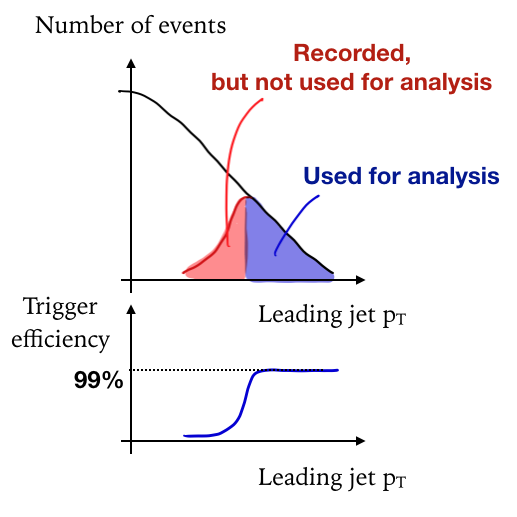
\includegraphics[width=0.28\textwidth]{figs_B2/efficiencySketch}
\caption{\color{black}\label{fig:wastedRate} \small Sketch of how trigger inefficiencies caused by a mismatch between the HLT and offline jet energy scales causes events to be recorded but never used for analysis.} %Trigger operation page
\vskip2pt
\end{center}
\end{wrapfigure}
\color{red}\textbf{Not sure the following should be here, but it's a good motivation to calibrate HLT objects in case someone isn't convinced. }\color{black} 
Differences in the energy scale of HLT and offline objects also lead to inefficiencies in the trigger selection, as events that should pass the trigger are rejected due to HLT miscalibrations. 
As an example, the minimum $p_{\rm{T}}$ threshold applied to jets used in physics analysis is set to be higher than the HLT threshold due to these differences, leading to a substantial waste in terms of events that are recorded but not used for analysis, as shown in Fig.~\ref{fig:wastedRate}. 
Preliminary studies performed within my StG and with collaborators show that, due to the steeply falling jet energy spectrum, the amount of events that are recorded but never used by offline analysis can be as high as 60\% for certain trigger chains. 
The application of TLA-motivated improved calibration constants at the HLT during e.g. LHC technical stops (allowing sufficient time for the reoptimization of the trigger menu) will improve the fraction of useful data recorded and impact the overall ATLAS data taking strategies. 
%In WP1, my team and I will contribute to the simultaneous derivation of calibration constants for trigger and offline jets. 

\textbf{Performance evaluation} Once the reconstruction and calibration algorithms are in place, their performance needs to be evaluated in data using figures of merit for probe objects such as response and resolution, tested against well-measured references. 
In WP2, we will prepare a comprehensive software toolkit for quantitative comparisons between physics objects reconstructed in TLA, TLA+PEB and offline, using automated problem detection techniques. 
This toolkit will be deployed online, so that HLT problems can be corrected as early as possible, and used offline to determine the performance of HLT objects.  
The extent to which a mismatch between tested object and reference objects requires intervention (e.g. modification of the reconstruction software, re-derivation of calibration constants...) varies depending on how this affects the sensitivity of WP3 and WP4 searches, estimated case by case as discussed in Sec.~\ref{sec:SensitivityStudies}.
 
\subsection{Specific methodologies for WP1: data compression}
\label{sub:SpecificMethodsCompression}

Compressing data can lead to further gains in terms of reducing the storage requirements of TLA and TLA+PEB. 
For this reason, this proposal investigates using deep autoencoders for lossy data compression, in a forward-looking study targeting HL-LHC. 
Preliminary studies by a Lund engineering (LTH) student that I co-supervised have shown that compressing data using deep autoencoders could lead to large space savings for TLA data and ATLAS data and simulation as a whole, leading to compression factors of 2 with negligible performance loss in TLA data~\cite{ToBeCited}. %Eric's thesis 
The advantage of autoencoders over methods such as Principal Component Analysis is that they are able to learn non-linear correlations among the nodes, 
and that, once the network is trained, the compression is fast (order 2-5 $\mu s$), making them a good candidate to be used in the HLT (latency $\approx$ 300 $\mu$ s). 
Within this proposal, I will supervise Master's students that continue studying performance, implementation and characteristics of such networks, towards a test implementation in system that emulates a HLT computing node. 

%Autoencoders are neural network that implement an approximation to the identity $f(x) \approx x$ using hidden layers with a smaller dimensionality with respect to input and output layers. 
%The smallest-dimensionality hidden layer contains a compressed representation of of the original information. 
%This compressed representation can then be saved to storage instead of the original data format, along with the network implementing the identity. 
%A figure of merit of the fidelity of this identity is the “reconstruction error”. 
%Autoencoders are widely used as anomaly detection algorithms. They are first trained on large amounts of non-anomalous reference data, and then presented with new data. If the new data does not match the reference data, the reconstruction error will be large and can be used as figure of merit to spot anomalies. 

\subsection{Common methodologies: analysis and interpretation tools}
\label{sub:CommonMethodsAnalysisTools}

This section outlines the data analysis and reinterpretation methods that are common to the searches in WP2-4, mentioning specific details for each of the searches. 

\textbf{Sensitivity studies} Prior to starting any of the physics analyses in WP2-4, studies are needed to determine the sensitivity of the analysis and refine the parameter space to be targeted (e.g. for producing fully simulated signal grids). 
These studies are implemented as a simplified version of the analysis, where trigger, detector and calibration effects are implemented using parameterizations and only employ full simulation wherever needed. 
For the implementation of the analyses in this proposal, we will use the RIVET software~\cite{ToBeCited}%RIVET 
as a starting point to analyze generator-level signal and background simulation. 
The advantage of using RIVET is that it easily interfaces with the CONTUR software~\cite{ToBeCited}%CONTUR
which allows to use a large number of LHC measurements to constrain new phenomena. 
This is particularly crucial for the searches in WP4, since measurements of jet fragmentation can already constrain dark QCD showering parameters. 
Sensitivity studies also provide a first testing ground for analysis techniques prior to data taking, and can be used during the data processing stage 
to understand the level of precision needed for HLT objects in order to be sensitive to certain kinds of signals. 

\textbf{Background reduction and estimate}
Standard Model backgrounds to all searches in WP2-WP4 need to be reduced and estimated. 

The background reduction techniques employed for the searches in WP2-4 select events based on one or more variables that discriminate signal from background.
These selections will be initially determined in simulation samples, and verified in “validation regions” with limited amounts of signal contamination. 
Simplicity is a driving factor in the choice of background reduction techniques in this proposal. 
Simpler selections allow searches to remain relatively agnostic to the specific model details, and ease the reinterpretation of our results using models others than the ones we employed, enabling the dissemination objectives in WP5. 
In the searches in WP2 and WP3, we will use the angular distribution of the jets as a discriminant between s-channel processes over the QCD backgrounds. 
In the semi-visible and composite jets searches in WP4, we will apply loose selection to reduce the QCD background already at the HLT. 
We will investigate the use and CPU cost of particle flow jet properties~\cite{ToBeCited}, %PFlow in ATLAS
event shape variables~\cite{ToBeCited}, %event shapes in ATLAS
jet substructure techniques and variables~\cite{ToBeCited}, %Nachman/Moult review, but also ttbar rejection
as well as new dedicated theoretical and phenomenological metrics for measuring QCD jet showering and identifying anomalies~\cite{ToBeCited}. %Lund plane, Thaler distance
To complement this \textit{cut-based} approach and to further increase the generality of the searches in WP4, exploratory studies will be performed in the direction of detecting anomalies over the known QCD background using ML techniques. % employing the same tools as for data compression in WP1. 
This will benefit from the work done within my VR Project Grant, which focuses on unsupervised search strategies specifically targeting resonance searches.

The estimation of the backgrounds, first tested in simulated data, will be derived directly from data wherever possible. 
The background of the dijet and dijet+ISR TLA searches in WP2 and WP3 will be derived directly from data, since the enormous number of events collected excludes the possibility of generating and simulating an equivalent amount, and because QCD simulations are subject to large theoretical and modeling uncertainties.  
For the semi-visible and lepton-in-jets searches in WP4, we will use a combination of data-derived and simulation-driven backgrounds, depending on whether the backgrounds are mainly from QCD (e.g. fake leptons, jets containing heavy flavor quarks decaying leptonically) or from QED and weak interactions (e.g. Z/W+jets where the vector boson decays into leptons and neutrinos, boosted top quarks containing a lepton from the W decay). 
Three background estimation methods are foreseen for the searches in this project: 
\begin{itemize}
\item For searches in WP2 and WP3 will estimate the smoothly falling QCD background with a functional form or with a continuous parameterization that does not accommodate narrow local excesses such as those from a new resonant particle. The experience gained with the high-statistics Run-2 dijet TLA search within my StG will be crucial to choose the appropriate method among a number of available techniques~\cite{ToBeCited}. %GaussianProcesses,FitMethod
\item For searches in WP4, we will use the ABCD method (e.g. Ref.~\cite{ToBeCited}) %ABCD
to estimate the background events in the signal region from normalization and control regions that have a minimal background contamination, defined in terms of independent variables. 
\item For the smaller W/Z backgrounds in the WP4 searches, we will make use of MC simulation using normalization factors derived from control regions in data. 
\end{itemize}
The robustness of the background estimation techniques will be evaluated in partial data scaled to the full expected dataset, using signal injection studies. 

\textbf{Cross-checks of performance within the analysis selection} The performance of the physics objects in the search will be monitored using the WP2 toolkit, after applying the background reduction selection. 

\subsubsection{Statistical analysis} Analyses in this project will be blinded, meaning that the region of phase space or the distribution where a signal is expected is not analysed until the full analysis strategy has been verified from data. We will use control regions and limited amounts of data where a signal would not have a significant impact to disentangle performance issues. 
Before unblinding the signal region, we will finalize background estimation, systematic uncertainties and expected limits satisfactorily, according to an internal peer-review committee. 
Once this is done, a statistical test will be employed to compare the observed data and estimated background. In this phase, we will also incorporate the systematic uncertainties from the reconstruction and calibration and on the background estimation techniques. 
Given the data-driven nature of the background estimation employed, the systematic uncertainties will mostly impact the signal yields and therefore have a limited impact on the search sensitivity. 
The statistical compatibility of background and data can then be extracted from either the CLs technique~\cite{ToBeCited}, %CL, from ERC StG
or from tests that are well suited for looking for a resonance or for an excess in the tails of the distribution, such as the BumpHunter and TailHunter~\cite{ToBeCited}. %Bumphunter/Tailhunter from ERC StG
We will use a statistical toolkit that enables sharing the final likelihood function, e.g. pyhf~cite{ToBeCited}. %pyhf

\subsubsection{Interpretation and dissemination of results} The outcome of the statistical analysis will be either compatibility between the data and the background estimation, or an excess above the background. In both cases, the implementation of the analysis code will be available via RIVET/RECAST/REANA and within the ESCAPE software catalogue, and the digitized results will be made available on HEPData~\cite{ToBeCited}. %Rivet
%Note: check that REANA is described somewhere beforehand

\textit{Null result:} The compatibility of data and background indicates that no new phenomena are found within the dataset used for the search. 
Therefore, constraints can be set on benchmark models in the limit setting phase. 
Frequentist or Bayesian techniques~\cite{ToBeCited} %BAT
can be used to set limits on the maximum allowed cross-section of the benchmark process versus the model parameters, e.g. the mass of new resonances. 
To extend the results of these searches to any resonant particle, we will also set limits on generic Gaussian-shaped resonances of different widths as done in all the dijet searches in my StG, and a responsibility of one of the students for the Run-2 dijet+ISR search~\cite{ToBeCited}. %dijet+ISR 
The outcomes of these searches will be plotted alongside results of other LHC searches and non-LHC experiments within a common theoretical framework. 
For WIMP searches, this will initially follow the methodology of Ref.~\cite{ToBeCited}, %DMWG invisible/visible searches
and will evolve following input from the broader community (e.g. from dedicated discussion within workshops and iDMEU). 

\textit{Discovery:} If an excess above the background prediction is observed, it will need to be characterized. 
Following the procedure for blind analyses, the observation will be made public as soon as the excess has been reviewed by the entire ATLAS Collaboration. 
It will be cross-correlated with other ATLAS searches which might see hints of the same process in different final states. 
Identifying the source of the excess and the nature of the resonance (e.g. distinguishing its parton content~\cite{ToBeCited}) %Vignaroli / Sanz
will become an outmost priority for the team~\footnote{This may lead to changes in the and work sharing of this project, as the entire team will be working first-hand with the tools and datasets employed up to that point for a result that has a world-wide impact on the field.} and for the Collaboration. 
In this case, the results of astrophysics and non-LHC experiments will be crucial to ascertain whether these results can be attributed to processes involving DM.

\subsection{Project planning}
\label{sub:ProjectPlanning}


%%%%%%BEGIN TO COMPILE UP TO HERE 
\clearpage
\begingroup
    \setboolean{inbibliography}{true}
\bibliographystyle{LHCb}
    \linespread{0.9}\selectfont
\bibliography{researchrefs}
\endgroup
%{\bf Note:} The PI is an author of Refs.~\cite{LHCb-PUB-2014-027,Bourgeois:2018nvk} and all the LHCb collaboration papers, with particular contributions to  Refs.~\cite{Aaij:2014jba,CERN-LHCC-2014-016,Aaij:2013mga,Aaij:2014ywt,LHCb-PUB-2014-040,Aaij:2016kjh,Aaij:2017lff}.
%The PI is acknowledged in Ref.~\cite{Jung:2014jfa}.
\end{document}  
%%%%%%END TO COMPILE UP TO HERE 

%This needs a study
%An example of a planned step in this direction is the possibility to change in the baseline choice of the main L1 trigger seeding jet TLAs from Run-2. 
%In Run-2, the TLA stream contained all events where there was at least one jet above a certain transverse momentum threshold at L1. 
%The Run-3 TLA stream will contain events where the selection is made on the sum of the transverse momentum of the jets in the event.
%This choice leads to a similar rate as the Run-2 one, thanks to the planned hardware improvements in the L1 trigger, but allows more flexible searches 



\subsubsection{Performance evaluation}
\ref{sec:Performance}



\subsubsection{Data compression}




%%%%
%%%%
